\chapter{The \lhcb\ experiment}
\label{chap:intro:lhcb}

The \lhcb\ experiment~\cite{Alves:2008zz,Aaij:2014jba} comprises a 
collaboration of around one thousand scientists and engineers, and a particle 
detector situated at point 8 of the \cern\ \ac{LHC}.
The general goal of the experiment is to explore the area of heavy flavour 
physics, that is the interactions of charm and beauty quarks and particles that 
contain them, and in particular to make the most precise measurements of heavy 
flavour properties to date, and to discover decays that were not observed by 
previous experiments.
Heavy flavour has a rich phenomenology: neutral particles can oscillate between 
their matter and antimatter states in flight, such as $\PBds \leftrightarrow 
\APBds$ and $\PDzero \leftrightarrow 
\APDzero$~\cite{Abulencia:2006ze,Aaij:2012nva}; bound states of four or five 
quarks can form~\cite{Aaij:2014jqa,Aaij:2015tga}; and they exhibit distinct 
matter-antimatter 
asymmetries~\cite{Aubert:2001nu,Abe:2001xe,Aaij:2012kz,Aaij:2013iua,Aaij:2016cla}.
With this, the \lhcb\ detector must be flexible enough to accommodate a wide 
physics programme.
This \namecref{chap:intro:lhcb:physics} will link the properties of heavy 
flavour decays with the requirements imposed on the detector if these 
properties are to be studied.

% TODO in order of importance:
% heavy flavour at LHC is forward -> detector is forward
% heavy flavour travels measurable distance -> measure it
% heavy flavour decays to hadrons -> PID

% Measure properties of HF
%   * Lifetimes
%   * Masses
%   * CP violation observables
%   * Production rates

At the \ac{LHC}, heavy flavour quarks are primarily produced through 
gluon-gluon fusion, illustrated in 
\cref{fig:intro:lhcb:hf_production:gg_fusion}.
With this mechanism, \bbbar\ and \ccbar\ pairs are predominantly produced in 
the forward region, at low angles to the beam, as shown in 
\cref{fig:intro:lhcb:hf_production:bbbar_angles}
To exploit this, the \lhcb\ detector is instrumented in the pseudorapidity 
region $2 < \Eta < 5$.
Particles produced in this region are highly boosted in the laboratory frame, 
and so given the lifetimes of the weakly decay heavy hadrons, of order of 
$0.1$--$\SI{1}{\pico\second}$, they can fly several millimetres before 
decaying.
With a sufficiently sensitive detector, such secondary vertices can be 
spatially distinguish from the primary proton-proton interaction vertices, 
providing a powerful discriminant between signal and background.
A good secondary vertex resolution also allows for a good decay time 
resolution, which is necessary for measuring the fast oscillations of \PBds\ 
and \PDzero mesons, and for measuring any possible decay time asymmetries.
In addition, the large displacement of the decay vertices with respect to the 
\ac{PV} causes the particles produced at the vertex to have a high \ac{IP}, 
defined in \cref{fig:intro:lhcb:vertexing} as the smallest transverse distance 
from the particle trajectory to the \ac{PV}.
A sufficient experimental resolution on the \ac{IP} would allow for additional 
discrimination between random tracks in the event and those from heavy flavour 
decays.
design of the \lhcb\ detector is particular optimised for the precise 
reconstruction of primary and second vertices, which itself requires a very 
good track reconstruction.

The properties of heavy flavour hadrons, such as their masses and lifetimes, 
can be inferred by reconstructing the four-momenta of their decay products, and 
so \lhcb\ aims to fully reconstruct the decays of beauty and charm hadrons, 
such as $\decay{\PBz}{\PKplus\PKminus}$, $\decay{\PBs}{\PDspm\PKmp}$ with 
$\decay{\PDsplus}{\PKminus\PKplus\Ppiplus}$, 
$\decay{\PLambdab}{\PJpsi\Pproton\PKminus}$ with 
$\decay{\PJpsi}{\Pmuon\APmuon}$, and $\decay{\PDz}{\PKplus\Ppiminus}$.
It is important to note that specific final states offer higher sensitivities 
to physics observables than others, and so it is crucial for \lhcb\ to be able 
to distinguish between different particle species.
For example, the decay $\decay{\PDz}{\PKplus\Ppiminus}$ is of the order of one 
thousand times less likely than the decay $\decay{\PDz}{\PKminus\Ppiminus}$, 
and so a poor \ac{PID} performance would result in a search for the 
$\PKplus\Ppiminus$ final state being swamped by $\PKminus\Ppiplus$.
In general, misidentification cannot be excluded completely, and so in addition 
a high momentum resolution is required to be able to distinguish between 
different final states in the parent mass spectrum.

An example of power of, and necessity for, good particle identification and 
momentum resolution is shown in \cref{fig:intro:lhcb:pid_power}.
Here, the signal decay is \decay{\PBzero}{\pimpip}, and the distributions are 
the two-body invariant mass before \ac{PID} requirements are made on the 
tracks~(\ref{fig:intro:lhcb:pid_power:pre}) and 
after~(\ref{fig:intro:lhcb:pid_power:post}).
As can be seen, before the requirements the distribution is dominated by other 
two-body \PBzero, \PBs, and \PLambdab\ decays, however after the backgrounds 
are almost entirely removed.
The presence of such backgrounds significantly increases the complexity of an 
analysis and can reduce the precision of the measurement.

In the following, the construction of the detector will be described, as 
motivated by the physics goals of the collaboration and the properties of heavy 
flavour outlined above.

\begin{figure}
  \begin{subfigure}[b]{0.4\textwidth}
    \centering
    \feynmandiagram [large, horizontal=a to b] {%
  i1 [particle=\(\Pgluon\)] -- [gluon] a -- [gluon] i2 [particle=\(\Pgluon\)],
  a -- [gluon, edge label=\(\Pgluon\)] b,
  f1 [particle=\(\APquark\)] -- [fermion] b -- [fermion] f2 [particle=\(\Pquark\)],
};

    \caption{Quark pair production}
    \label{fig:intro:lhcb:hf_production:gg_fusion}
  \end{subfigure}
  \begin{subfigure}[b]{0.6\textwidth}
    \begin{tikzpicture}
  \node[anchor=south west, inner sep=0] (image) at (0, 0) {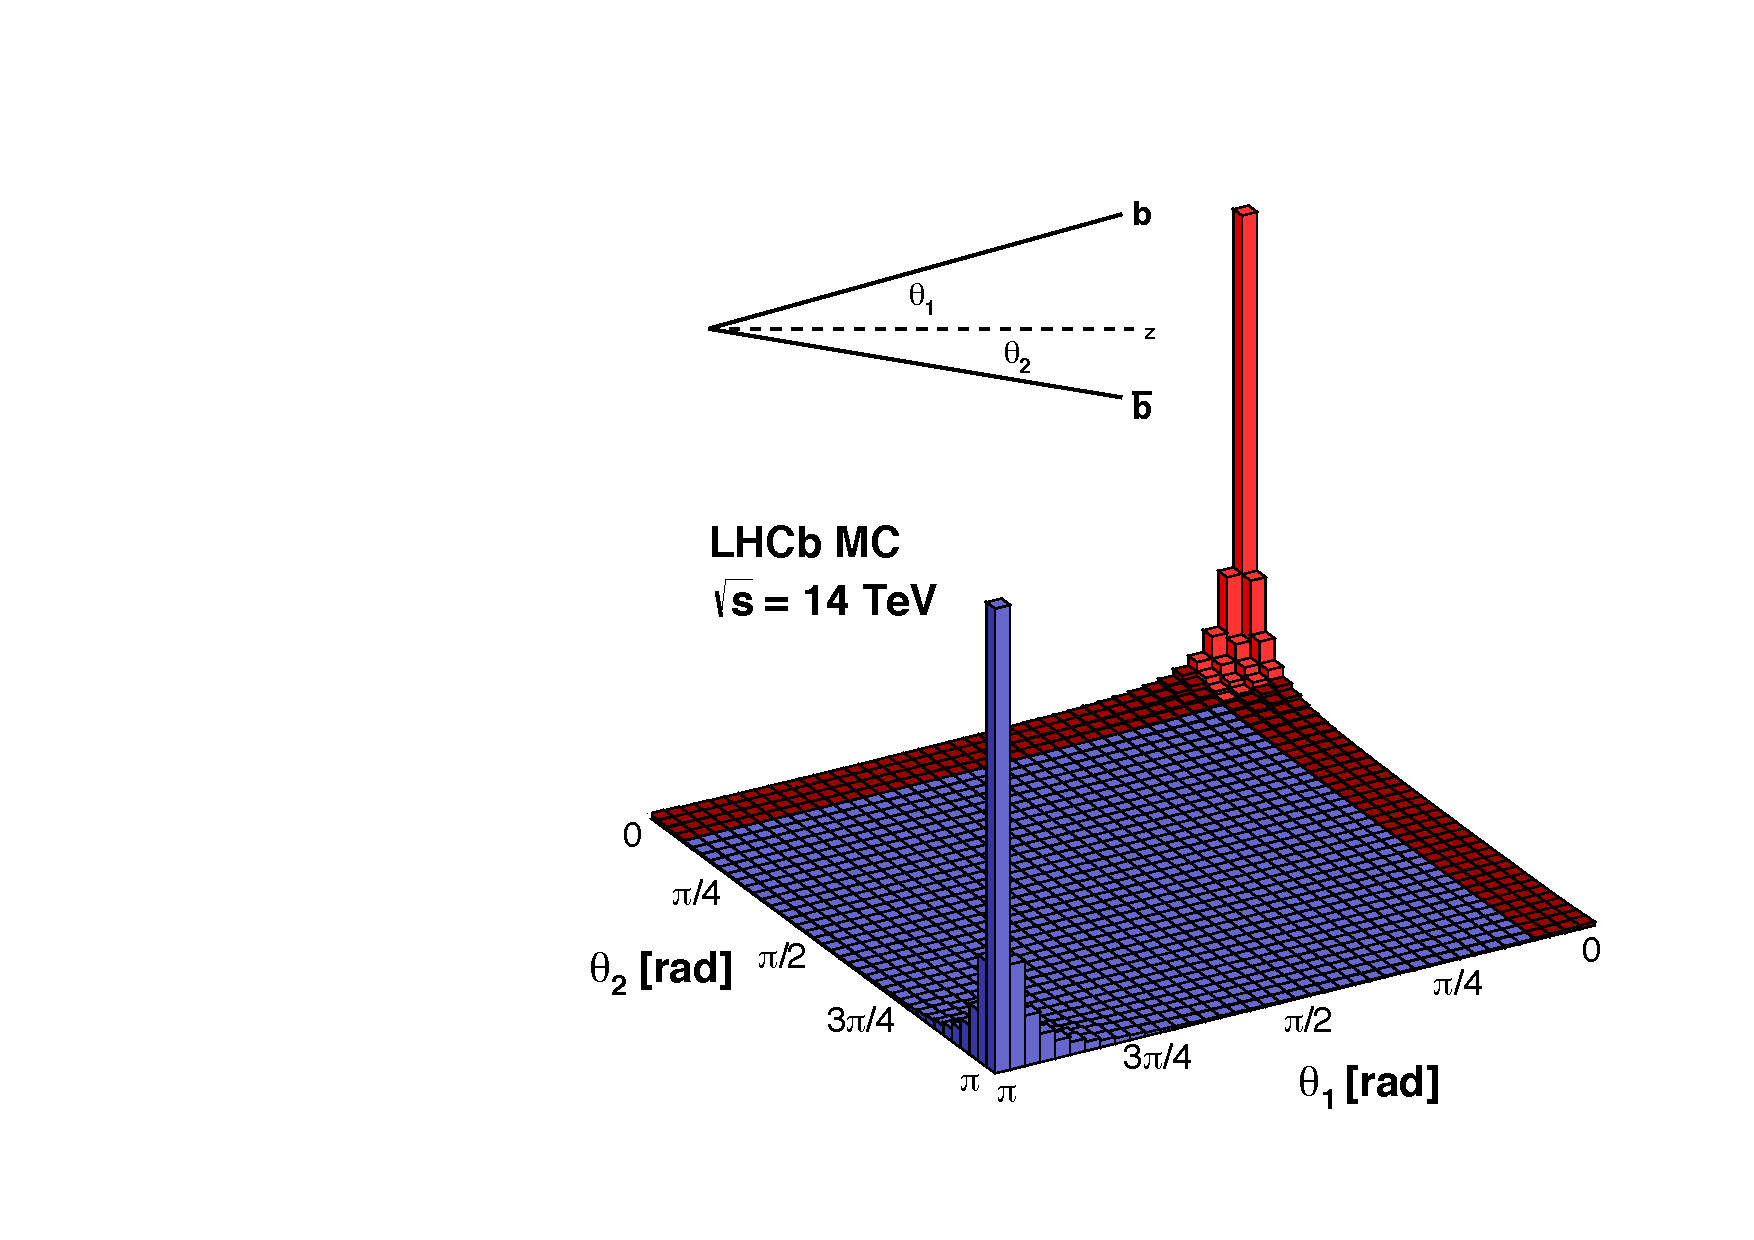
\includegraphics[width=\textwidth]{introduction/bbbar_production_angles}};
  \begin{scope}[x={(image.south east)}, y={(image.north west)}]
    % Grid to help find coordinates on the image
    % \draw[step=0.02, gray, very thin] (0, 0) grid (1, 1);
    % Box to cover axis labels
    \path[fill=white] (0.02, 0.16) rectangle (0.18, 0.22) node [pos=0.5] {\footnotesize$\theta_{1}$};
    \path[fill=white] (0.64, 0.06) rectangle (0.78, 0.12) node [pos=0.5] {\footnotesize$\theta_{2}$};
    % Box to cover angle definitions
    \path[fill=white] (0.14, 0.66) rectangle (0.54, 0.88);
    % Box to cover 'LHCb MC' label
    \path[fill=white] (0.14, 0.48) rectangle (0.36, 0.58);
  \end{scope}
\end{tikzpicture}

    \caption{$\Pbottom\APbottom$ production distribution}
    \label{fig:intro:lhcb:hf_production:bbbar_angles}
  \end{subfigure}
  \caption{%
    Feynman diagram of quark pair production via gluon-gluon fusion 
    (\subref*{fig:intro:lhcb:hf_production:gg_fusion}), and a simulation of the 
    angular distribution of \bbbar\ production at the \ac{LHC} at $\sqrt{s} = 
    \SI{13}{\TeV}$ (\subref*{fig:intro:lhcb:hf_production:bbbar_angles}).
  }
  \label{fig:intro:lhcb:hf_production}
\end{figure}

\begin{figure}
  \begin{subfigure}[b]{0.5\textwidth}
    \centering
    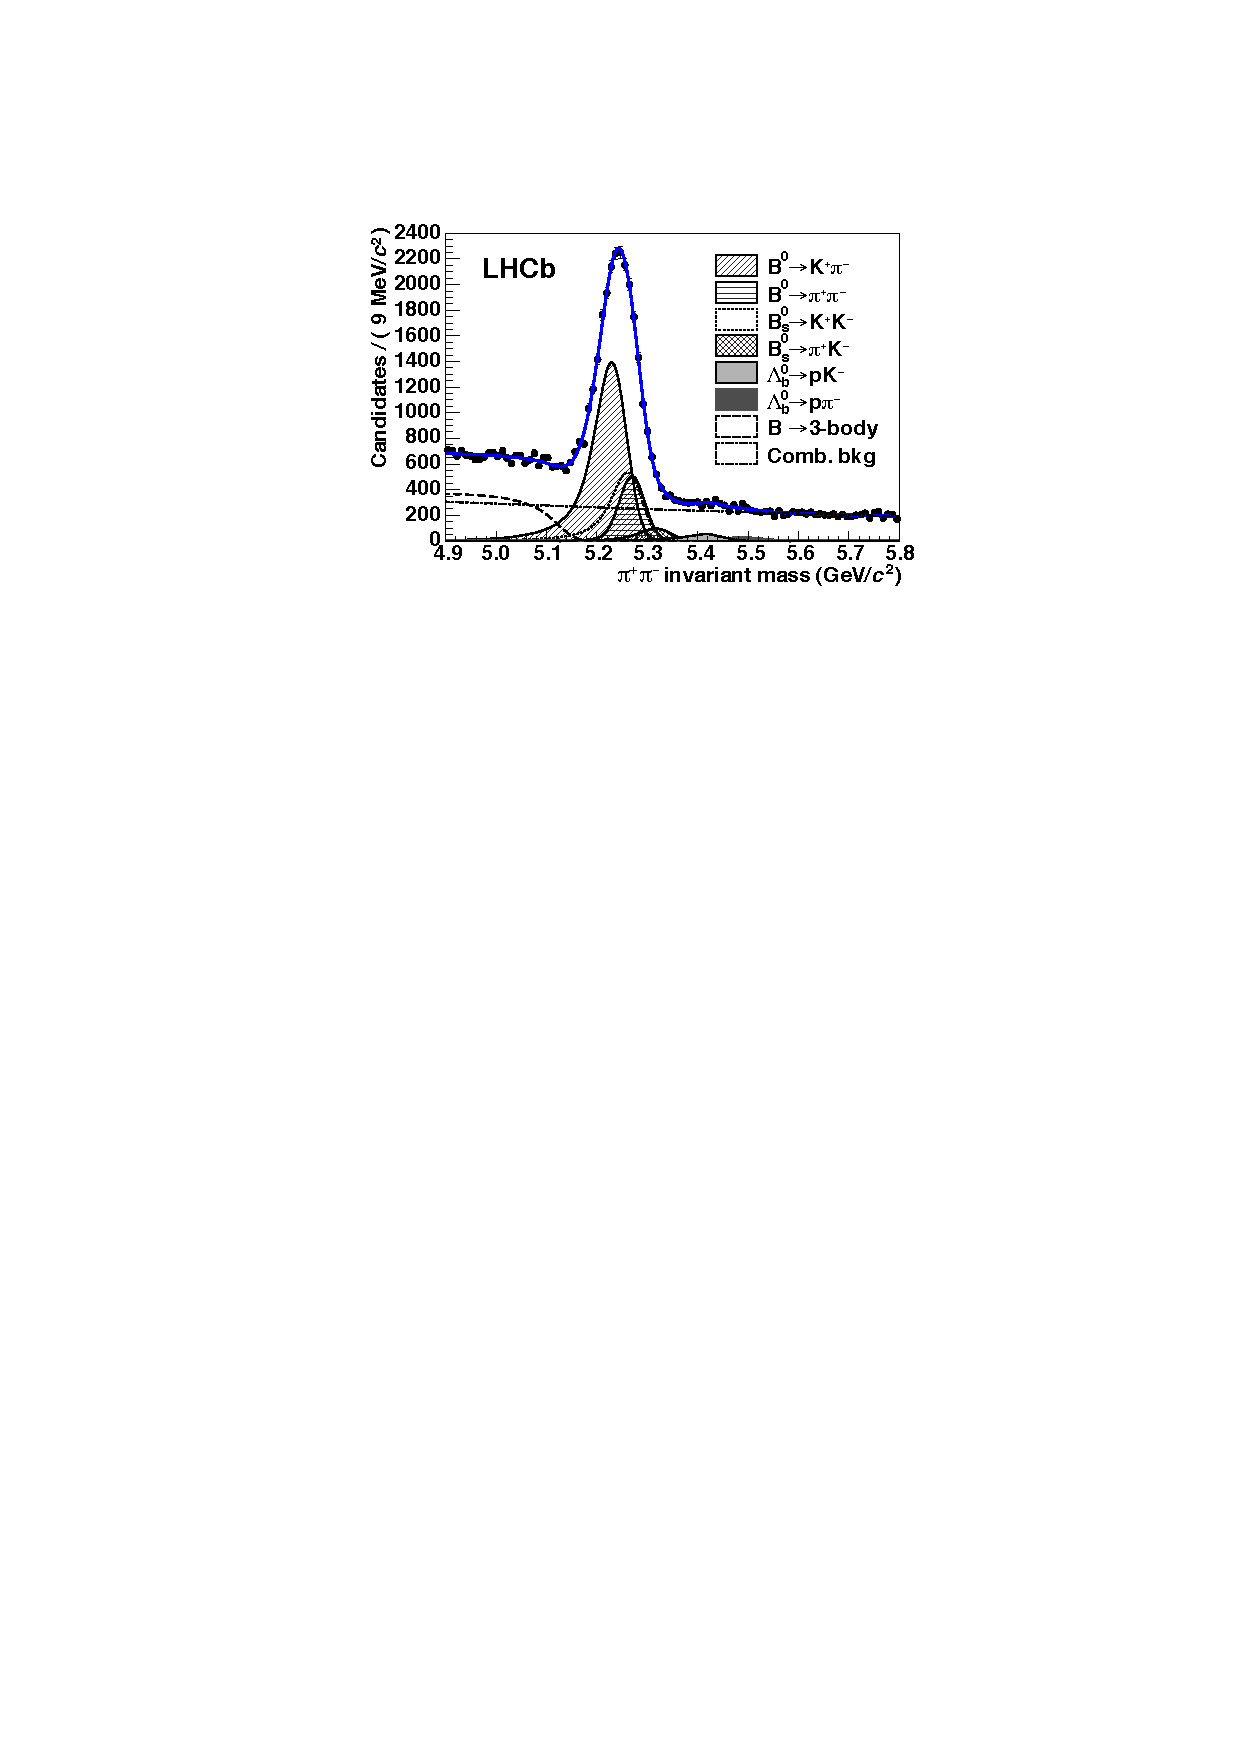
\includegraphics[width=\textwidth]{introduction/B2pipi_pre_pid}
    \caption{Before \ac{PID} requirements}
    \label{fig:intro:lhcb:pid_power:pre}
  \end{subfigure}
  \begin{subfigure}[b]{0.5\textwidth}
    \centering
    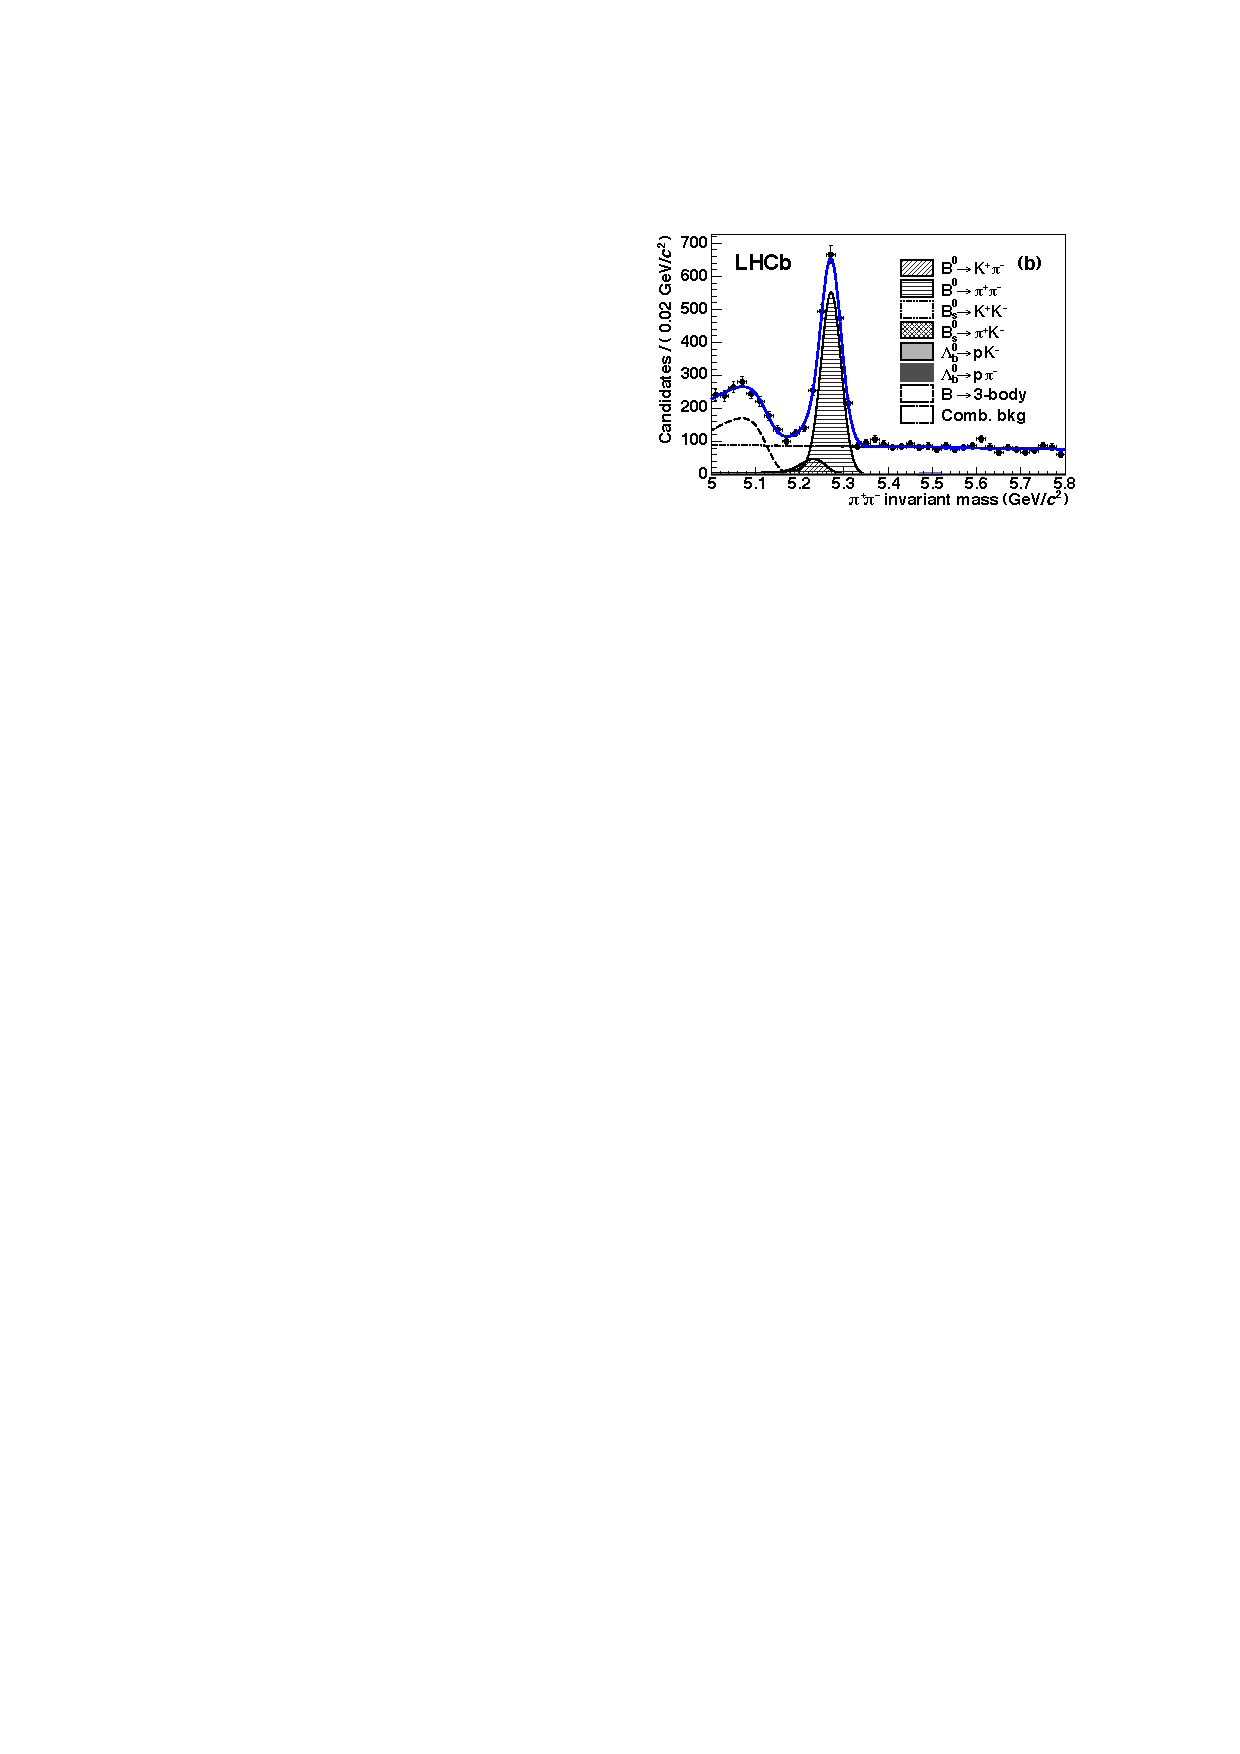
\includegraphics[width=\textwidth]{introduction/B2pipi_post_pid}
    \caption{After \ac{PID} requirements}
    \label{fig:intro:lhcb:pid_power:post}
  \end{subfigure}
  \caption{%
    Two-body invariant mass spectrum, under the $\pimpip$ hypothesis, 
    before~(\subref*{fig:intro:lhcb:pid_power:pre}) and 
    after~(\subref*{fig:intro:lhcb:pid_power:post}) \ac{PID} 
    requirements~\cite{Aaij:2012as}.
    The contribution from the signal decay is hatched with horizontal lines.
  }
  \label{fig:intro:lhcb:pid_power}
\end{figure}

\section{Detector}
\label{chap:intro:lhcb:detector}

Within the \lhcb\ experiment, the co-ordinate system is defined such that the 
$z$-axis is aligned along the beam direction, increasing in the clockwise 
direction along the \ac{LHC} ring; the $y$-axis is aligned with gravity, 
increasing away from the Earth's surface; and the $x$-axis, defined as $x = y 
\times z$, is then increasing away from the centre of the accelerator.
In this \namecref{chap:intro:lhcb:detector}, and in all that follows, this 
coordinate system will be used.

The detector is shown in \cref{fig:intro:lhcb:detector}.
Its forward geometry is evident, roughly forming a cone between 10 and 
\SI{400}{\milli\radian} in the polar angle $\theta$, or equivalently $2 < \Eta 
< 5$.
A dipole magnet with an integrated field strength of \SI{4}{\tesla\metre} bends 
charged particle trajectories in the $xz$ plane, with the trajectories 
themselves being recorded by the tracking system.
This comprises a vertex detector centred around the proton-proton interaction 
region, three planes of tracking stations before the magnet, and three planes 
after.
Immediately downstream of the vertex detector, increasing is $z$, in the first 
of two \ac{RICH} detectors, used for particle identification, the second of 
which is after the tracking stations downstream of the magnet.
After this, a calorimetry system is in place to identify neutral particles such 
as the \Ppizero\ and the photon, as well as to measure their energy and that of 
the charged particles.
Finally, a muon system is installed after the calorimeters, which is used for 
muon identification.

The data recorded by the detector is selected in real time by a hardware 
trigger, after which a software triggers performs an event reconstruction.
There are not enough computing resources available to the experiment to record 
and analyse every proton-proton bunching crossing, and so the trigger is as 
important to achieving the physics goals of the collaboration as the detector, 
as it is responsible for deciding which crossings should be kept and which 
should be discarded.

Each sub-detector shall now be described in turn, followed by a description of 
the trigger system and how the detector was upgraded in between \runone\ to 
\runtwo.

\begin{figure}
  \centering
  \begin{tikzpicture}
  % Use trim and crop to remove some of the white space around the image
  \node[anchor=south west, inner sep=0] (image) at (0, 0) {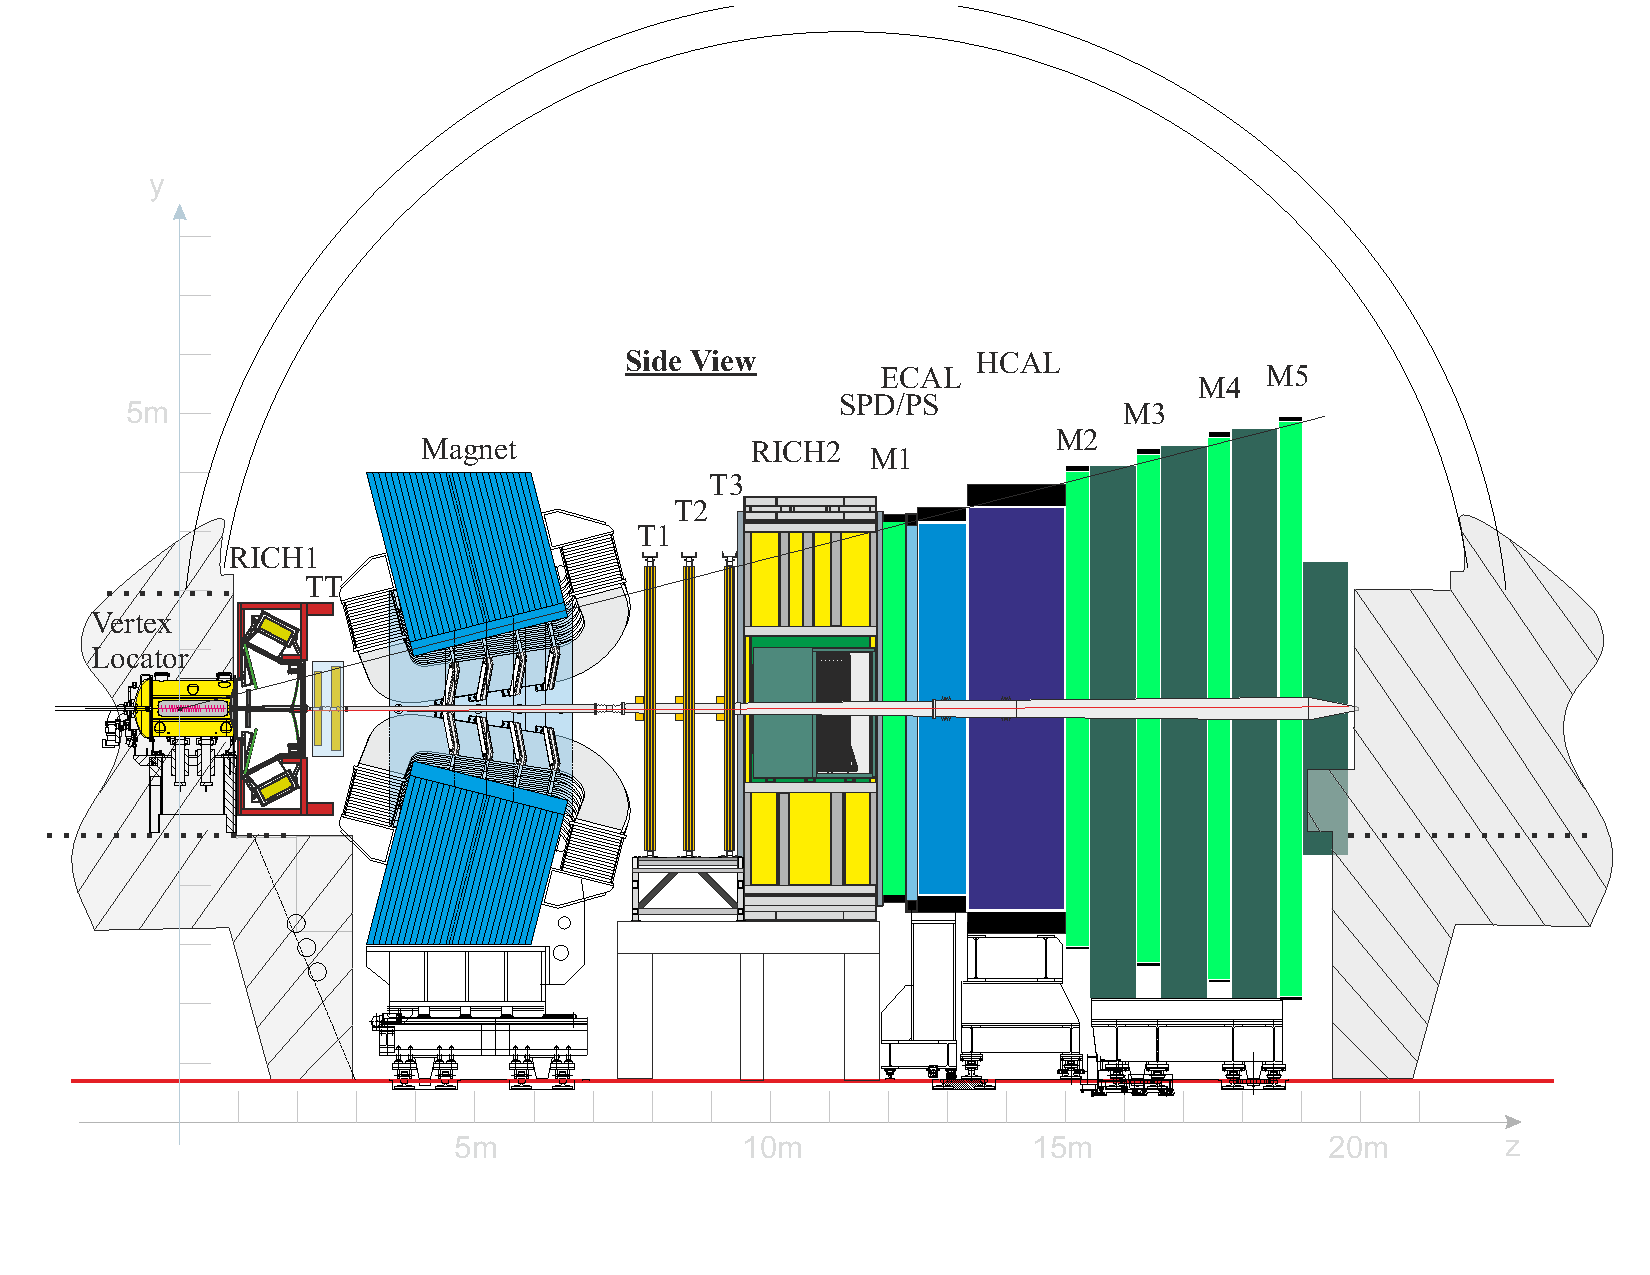
\includegraphics[width=\textwidth, trim={1cm 1.7cm 0.5cm 3cm}, clip]{introduction/lhcb_detector}};
  \begin{scope}[x={(image.south east)}, y={(image.north west)}]
    % Grid to help find coordinates on the image
    % \draw[step=0.02, gray, very thin] (0, 0) grid (1, 1);
    % Box to cover "Side View" label
    \path[fill=white] (0.36, 0.78) rectangle (0.46, 0.84);
  \end{scope}
\end{tikzpicture}

  \caption{%
    A schematic of the \lhcb\ detector.
    In this Figure, the $z$-axis, labelled, increases from left to right, the 
    $y$-axis, also labelled, increases from bottom to top, and the $x$-axis 
    increases into the page.
  }
  \label{fig:intro:lhcb:detector}
\end{figure}

\subsection{Tracking}
\label{chap:intro:lhcb:detector:tracking}

Charged particle trajectories are reconstructed as tracks using hits left in 
the tracking system.
This comprises the vertex locator~(\velo) centred around the proton-proton 
interaction region, the Tracker Turicensis~(\ttracker) before the magnet, and 
the T-stations after the magnet.
In \runone, the tracking system achieved a momentum resolution 
$\unc{\ptot}/\ptot$ from $0.5\%$ at $\ptot = \SI{5}{\GeVc}$ to $0.8\%$ at 
\SI{100}{\GeVc}, and a track \acl{IP} resolution varying from around 
\SI{70}{\micro\metre} for tracks with a low \pT\ to \SI{20}{\micro\metre} at 
high \pT.

The \velo\ is an extremely precise silicon strip detector, whose active 
elements come as close as \SI{8}{\milli\metre} away from the \ac{LHC} beams.
Two sets of 24 silicon modules are arranged either side of the beam, each of 
which measures particle hits in $r$ and $\phi$ coordinates.
Charged particles traversing the active silicon can ionise the material, 
creating electron-hole pairs that drift towards the electrodes, registering a 
hit as an electrical signal.
The magnetic field strength inside the \velo\ is approximated to be zero, and 
so track segments are reconstructed as straight lines using the hits in the 
sensors.
So-called long tracks, the track type used for the majority of physics 
analyses, are created by combining \velo\ segments with hits in the T-stations 
after the magnet.

The three T-stations, T1--3, each comprise a silicon strip detector close to 
the beam pipe~(the \itracker) and a drift-tube detector in the outer 
regions~(the \otracker).
The \itracker\ has a finer spatial resolution than the \otracker, and covers a 
small area around the beam where the particle multiplicities are particularly 
high.
The \otracker\ covers an area of approximately \SI{30}{\metre\squared}, about 8 
times greater than that covered by the \itracker.
Ionising particles free electrons from the gas molecules within the tubes, 
which are detected by anode wires and registered as hits.
The point of ionisation within the wire is determined by measuring the electron 
drift time, improving the track momentum resolution.
This is further improved by adding the hits detected in the \ttracker, upstream 
of the T-stations.
The \ttracker\ is a silicon strip detector of the same technology as the 
\itracker, with the three stations covering a total area of around 
\SI{8}{\metre\squared}.

The tracking efficiency, the fraction of real tracks that are formed given 
enough hits were deposited to form one, is measured using a tag-and-probe 
technique with \JpsiTomumu\ decays, which will be explained in more detail in 
\cref{chap:prod:effs:tracking}.
The formation of tracks assumes that the tracker system is perfectly aligned, 
but the positions of the various stations can change with time.
To compensate for this effect, alignment constants are computed periodically 
and used in the reconstruction software.
The effect of an improved alignment is illustrated in 
\cref{fig:intro:lhcb:alignment}, where the $\Pmuon\APmuon$ mass resolution 
improves from \SI{92}{\MeVcc} with an initial alignment to \SI{49}{\MeVcc} with 
an improved one, that more accurately reflects the state of the 
detector~\cite{Dujany:082010}.
Without the improved alignment, it is harder to distinguish three distinct 
resonant states.

\subsection{Particle identification}
\label{chap:intro:lhcb:detector:pid}

In order to compute the invariant mass of a decay vertex, the mass of the 
tracks forming that vertex must be known.
As each long-lived charged particle has a unique mass, the mass measurement 
assigns an identity to that track, in the process of \acf{PID}.
Through the momentum-velocity relation, the mass of a particle can be 
determined by combining the momentum measurement from the tracking system with 
a velocity measurement.

Tracks created by pions, kaons, and protons are identified using the response 
of two \acl{RICH} detectors: \richone\ located upstream of the magnet; and 
\richtwo\ located downstream.
Electron and muon discrimination at a weaker level.
\richtwo has larger surface area than \richone\ but has a smaller angular 
acceptance, being designed to efficiently identify tracks with momenta in the 
range \SIrange{15}{100}{\GeVc} which largely occupy the low-$\theta$ region.
\richone\ is effective in the momentum range \SIrange{3}{60}{\GeVc}.
During \runone, \richone contained a mixture of aerogel and \ce{C4F10} gas, of 
which the former was removed before the start of \runtwo.
\richtwo\ contains \ce{CF4} gas.

As charged particles travels through one of these `radiators', each of 
refractive index $n$, they emit Cherenkov radiation if they are travelling 
faster than the phase velocity of light of the radiator.
This light is emitted at an angle $\thetac$ to the particle trajectory, and is 
related to the speed of the particle as
\begin{equation}
  \cos{\thetac} = \frac{1}{n\beta},
\end{equation}
where $\beta = v/c$.
The refractive indices of the radiators are known and are controlled by 
monitoring the gas pressure and temperature over time.
By measuring \thetac\ the \rich\ detectors can provide velocity measurements of 
charged tracks, and hence identify them.

Each Cherenkov light cone is detected as a ring of photons by planes of photon 
detectors arranged in arrays outside of the geometric acceptance of the \lhcb\ 
detector, after having been reflected by a set of spherical and plane mirrors.
In order to assign a particle mass hypothesis to a track, a maximum likelihood 
method is used~\cite{Forty:1998eqa}.
Initially, all reconstructed tracks are assumed to be pions, and the 
\emph{predicted} Cherenkov rings assuming this hypothesis set are projected 
onto the photo-detector planes within both \richone\ and \richtwo.
The value of the log-likelihood is computed by comparing the predicted number 
of photons within each photon detector to those observed.
For each track, the mass hypothesis is then changed to each of (\Pe, \Pmu, 
\Ppi, \PK, \Pproton), the rings assuming the new global hypothesis set are 
projected, and the log-likelihood is re-computed.
The hypothesis giving the largest increase in the log-likelihood is recorded, 
and the track hypothesis is returned back to its original value.
After all individual track hypotheses have been trialled, the single hypothesis 
change that gave the largest increase in the log-likelihood is applied to the 
respective track.
This procedure is repeated until the log-likelihood no longer increases with 
any change in the hypothesis set.
The outputs of this method are the \ac{DLL} variables, with one value per track 
for each of the (\Pe, \Pmu, \PK, \Pproton) hypotheses.
Each \ac{DLL} variable is defined as the difference in the log-likelihood value 
when the track mass hypothesis is changed from the pion hypothesis to the one 
of the variable, for example \dllkpi.

\subsection{Calorimetry}
\label{chap:intro:lhcb:detector:calo}

Given the momentum measurements from the tracking system and the mass 
measurements from the \ac{RICH} detectors, the particle energy is already 
determined.
For hadrons then, a precise calorimetry system is not necessary.
However, the momentum and mass measurements are complex and require a 
significant amount of time to compute, and so cannot be used in the first stage 
of the trigger where the proton-proton collision rate must be reduced from 
\SI{40}{\mega\hertz} down to around \SI{1}{\mega\hertz}.
In addition, the \rich\ detectors are much less sensitive to electron \ac{PID} 
than (\Pe, \Pmu, \Pproton), and the tracking system cannot detect photons or 
neutral pions, and so additional detection methods are required.

To provide a fast positive trigger decision for events containing hadronic 
decays of heavy flavour, a hadronic calorimeter, the \hcal, is employed.
This is a sampling calorimeter, comprised of alternating layers of iron and 
active scintillating material and positioned downstream of \richtwo.
Hadrons traversing the \hcal\ deposit energy in these layers, with the 
scintillation light collected by plastic fibres and recorded by 
photo-multiplier tubes.
The \hcal\ is segmented transversely into square cells, \SI{130}{\milli\metre} 
in width near the beam and \SI{260}{\milli\metre} in width in the outer 
regions, decreasing in granularity to account for the lower particle 
multiplicities.
The total transverse energy \ET\ in all clusters of $2\times2$ cells is 
computed, and a positive trigger decision is made if the maximum \ET\ is above 
some threshold, typically between \SIrange{3.5}{3.7}{\GeV}.
The \hcal\ provides the highest rate of positive trigger decisions out of those 
at the first trigger level, giving a signal efficiency of around 
\SI{40}{\percent} for two-body \PB decays, and \SI{20}{\percent} for four-body 
\PD decays.
The resolution on the energy measured by the \hcal\ has been measured to be 
$\unc{E}/E = \SI{69 \pm 5}{\percent}/\sqrt{E}$ plus a constant term of \SI{9 
  \pm 2}{\percent}~\cite{Perret:2015pla}.

An electromagnetic calorimeter, the \ecal, is located in front of the \hcal, 
and measures the energies of electrons and photons.
It is made of longitudinally alternating transverse layers of lead and 
scintillator, throughout which run clear plastic fibres, collecting the 
scintillation light to be read by photo-multiplier tubes.
It is segmented in the transverse plane into three regions, increasing in 
granularity towards the beam.
The energy measurements it makes are used in the first trigger level to accept 
high \ET\ electrons and photons, and in the reconstruction of \Ppizero and 
\Peta mesons.
The ability to discriminate between electrons and photons in the trigger 
decision is provided by the scintillating pad/preshower detector~(\spd/\ps) 
which consists of two layers of near-identical scintillator either side of a 
\SI{15}{\milli\metre}-thick layer of lead~(\ce{Pb}) converter, transversely 
segmented in the same manner as the \ecal.
A positive electron trigger decision requires an \ET\ measurement of between 
\SIrange{2.5}{3.0}{\GeV} in a cluster of $2\times2$ cells in the \ecal, along 
with hits in both the \spd\ and the \ps\ pads in front of the corresponding 
\ecal\ cluster.  A positive photon trigger decision is near-identical to this, 
except that no hits must be present in the corresponding \spd\ cells.
The resolution on \ecal\ energy measurements are $\unc{E}/E = \SI{9 \pm 
  0.5}{\percent}/\sqrt{E}$, plus a constant term of 
\SI{0.8}{\percent}~\cite{Perret:2015pla}.

\subsection{Event selection}
\label{chap:intro:lhcb:detector:trigger}

\subsection{Data flow}
\label{chap:intro:lhcb:detector:dataflow}


\begin{figure}
  \centering
  % Draw perpendicular markers at line intersections
% http://tex.stackexchange.com/a/21759/45857
\tikzset{
  right angle quadrant/.code={
    \pgfmathsetmacro\quadranta{{1,1,-1,-1}[#1-1]}     % Arrays for selecting quadrant
    \pgfmathsetmacro\quadrantb{{1,-1,-1,1}[#1-1]}},
  right angle quadrant=1, % Make sure it is set, even if not called explicitly
  right angle length/.code={\def\rightanglelength{#1}},   % Length of symbol
  right angle length=2ex, % Make sure it is set...
  right angle symbol/.style n args={3}{
    insert path={
      let \p0 = ($(#1)!(#3)!(#2)$) in     % Intersection
      let \p1 = ($(\p0)!\quadranta*\rightanglelength!(#3)$), % Point on base line
      \p2 = ($(\p0)!\quadrantb*\rightanglelength!(#2)$) in % Point on perpendicular line
      let \p3 = ($(\p1)+(\p2)-(\p0)$) in  % Corner point of symbol
      (\p1) -- (\p3) -- (\p2)
    }
  }
}
\begin{tikzpicture}[
  x=2cm,
  y=2cm,
  axis/.style={very thick,->,gray},
  beam/.style={very thick,->,gray},
  scale=1.5,
  thick
  ]
  % Origin
  \coordinate (O) at (0, 0);
  % B decay vertex
  \coordinate (Bvtx) at (1, 0.5);
  % Offset of muon arrows, with respect to Bvtx
  \coordinate(mumoffset) at (0.3, 0.4);
  \coordinate(mupoffset) at (0.6, -0.2);
  % Compute the coordinates of the ends of the muon lines
  \coordinate (mum) at ($(Bvtx) + (mumoffset)$);
  \coordinate (mup) at ($(Bvtx) + (mupoffset)$);

  % Coordinate axes
  \draw[axis] (-0.6, -0.5) -- +(0.2, 0) node [below] {$z$};
  \draw[axis] (-0.6, -0.5) -- +(0, 0.2) node [left] {$y$};

  \draw[beam] (-1.0, 0) -- (-0.1, 0) node [below, at start] {$p$};
  \draw[beam] (1.5, 0) -- (0.1, 0) node [below, at start] {$p$};

  % D meson
  \draw[dashed, color=gray, text=black] (O) -- (Bvtx) node [above, pos=0.5] {\PDz};
  % Negative child
  \draw[->] (Bvtx) -- (mum) node [above] {\PKminus};
  \draw[dotted] (Bvtx) -- ($(Bvtx) - 3*(mumoffset)$) node [name=mumend] {};
  % Positive child
  \draw[->] (Bvtx) -- (mup) node [below] {\Ppiplus};
  \draw[dotted] (Bvtx) -- ($(Bvtx) - 2*(mupoffset)$) node [name=mupend] {};

  % Primary vertex
  \node[star,star points=10,draw=orange!50,fill=orange!20,inner sep=0pt,minimum size=0.4cm] at (O) {};

  % Negative muon IP
  \draw[right angle length=1mm, right angle symbol={Bvtx}{mumend}{O}] ($(Bvtx)!(O)!(mumend)$) -- (O) node [pos=0.2, left] {$\text{IP}_{\PKminus}$};
  % Positive muon IP
  \draw[right angle length=1mm, right angle symbol={Bvtx}{mupend}{O}] ($(Bvtx)!(O)!(mupend)$) -- (O) node [midway, left] {$\text{IP}_{\Ppiplus}$};
\end{tikzpicture}

  \caption{%
    Illustration of vertexing, showing a \PDz meson decaying in flight to a 
    kaon and a pion.
    The kaon and pion are reconstructed as tracks, and then the \PDzero decay 
    vertex is inferred from the point of closest approach of the two tracks.
    The minimum transverse distance the tracks make when extrapolated back 
    towards the primary proton-proton vertex, the \acf{IP}, is shown.
  }
  \label{fig:intro:lhcb:vertexing}
\end{figure}

\begin{figure}
  \begin{subfigure}{0.5\textwidth}
    \centering
    \begin{tikzpicture}
  \node[anchor=south west, inner sep=0] (image) at (0, 0) {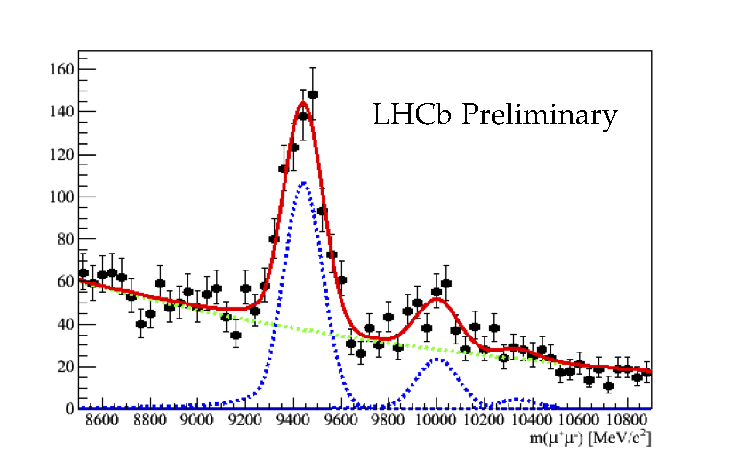
\includegraphics[width=\textwidth]{introduction/mumu_pre_alignment}};
  \begin{scope}[x={(image.south east)}, y={(image.north west)}]
    % Grid to help find coordinates on the image
    % \draw[step=0.05, gray, very thin] (0, 0) grid (1, 1);
    % Box to cover 'LHCb preliminary' label
    \path[fill=white] (0.5, 0.7) rectangle (0.85, 0.8);
  \end{scope}
\end{tikzpicture}

    \caption{Before}
    \label{fig:intro:lhcb:alignment:pre}
  \end{subfigure}
  \begin{subfigure}{0.5\textwidth}
    \centering
    \begin{tikzpicture}
  \node[anchor=south west, inner sep=0] (image) at (0, 0) {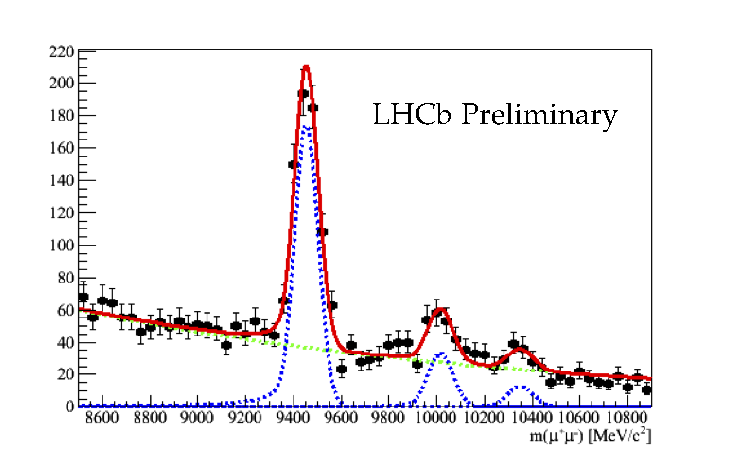
\includegraphics[width=\textwidth]{introduction/mumu_post_alignment}};
  \begin{scope}[x={(image.south east)}, y={(image.north west)}]
    % Grid to help find coordinates on the image
    % \draw[step=0.05, gray, very thin] (0, 0) grid (1, 1);
    % Box to cover 'LHCb preliminary' label
    \path[fill=white] (0.5, 0.7) rectangle (0.85, 0.8);
  \end{scope}
\end{tikzpicture}

    \caption{After}
    \label{fig:intro:lhcb:alignment:post}
  \end{subfigure}
  \caption{%
    Invariant mass distribution of $\Pmuon\APmuon$ candidates in the region of 
    the first three \PUpsilon resonances~\cite{Dujany:082010}.
    The left plot~(\subref*{fig:intro:lhcb:alignment:pre}) shows the data 
    reconstructed with a preliminary alignment, whilst the right 
    plot~(\subref*{fig:intro:lhcb:alignment:post}) shows the result of a 
    reconstruction performed with a revised alignment.
    The $\Pmuon\APmuon$ mass resolution improves from \SI{92}{\MeVcc} to 
    \SI{49}{\MeVcc}.
  }
  \label{fig:intro:lhcb:alignment}
\end{figure}
